%%%%%%%%%%%%%%%%%%%%%%%%%%%%%%%%%%%%%%%%%%%%%%%%%%%%%%%%%%%%%%%%%%%%%
%% This is a (brief) model paper using the achemso class
%% The document class accepts keyval options, which should include
%% the target journal and optionally the manuscript type.
%%%%%%%%%%%%%%%%%%%%%%%%%%%%%%%%%%%%%%%%%%%%%%%%%%%%%%%%%%%%%%%%%%%%%
\documentclass[journal=jpcbfk,manuscript=article]{achemso}

%\documentclass[english,aps,preprint,pre,floatfix,nofootinbib,showpacs,showkeys]{revtex4-1}
%%%%%%%%%%%%%%%%%%%%%%%%%%%%%%%%%%%%%%%%%%%%%%%%%%%%%%%%%%%%%%%%%%%%%
%% Place any additional packages needed here.  Only include packages
%% which are essential, to avoid problems later. Do NOT use any
%% packages which require e-TeX (for example etoolbox): the e-TeX
%% extensions are not currently available on the ACS conversion
%% servers.
%%%%%%%%%%%%%%%%%%%%%%%%%%%%%%%%%%%%%%%%%%%%%%%%%%%%%%%%%%%%%%%%%%%%%
\usepackage[version=3]{mhchem} % Formula subscripts using \ce{}

\SectionNumbersOn

%include hyperlinks to figures
%\documentclass{article}
\usepackage{graphicx}
\usepackage[%  
    colorlinks=true,
    pdfborder={0 0 0},
    linkcolor=black,
    citecolor=black,
    urlcolor=black
]{hyperref}

\usepackage{amsmath}
\usepackage{amssymb}
\usepackage{color}
\usepackage{CJK}
\usepackage{framed}
%\usepackage[hidelinks]{hyperref}
%\usepackage{algorithm}
%\usepackage{algpseudocode}
%\algdef{SE}[DOWHILE]{Do}{doWhile}{\algorithmicdo}[1]{\algorithmicwhile\ #1}

\usepackage[scaled=0.85]{beramono}
\usepackage[T1]{fontenc}
\usepackage{changepage}
\usepackage{mathrsfs}
\usepackage{comment}
\usepackage[normalem]{ulem}
\usepackage{algorithm}
\usepackage{subfig}
\usepackage{algpseudocode}

%%%%%%%%%%%%%%%%%%%%%%%%%%%%%%%%%%%%%%%%%%%%%%%%%%%%%%%%%%%%%%%%%%%%%
%% If issues arise when submitting your manuscript, you may want to
%% un-comment the next line.  This provides information on the
%% version of every file you have used.
%%%%%%%%%%%%%%%%%%%%%%%%%%%%%%%%%%%%%%%%%%%%%%%%%%%%%%%%%%%%%%%%%%%%%
%%\listfiles

%%%%%%%%%%%%%%%%%%%%%%%%%%%%%%%%%%%%%%%%%%%%%%%%%%%%%%%%%%%%%%%%%%%%%
%% Place any additional macros here.  Please use \newcommand* where
%% possible, and avoid layout-changing macros (which are not used
%% when typesetting).
%%%%%%%%%%%%%%%%%%%%%%%%%%%%%%%%%%%%%%%%%%%%%%%%%%%%%%%%%%%%%%%%%%%%%

\makeatletter
    \setlength\@fptop{0\p@}
\makeatother

\newcommand*\mycommand[1]{\texttt{\emph{#1}}}

\newcommand{\state}[1]{$\mathcal{S}_{#1}$}
\newcommand{\Expect}[1]{\mathrm{E}\left[#1\right]}
\newcommand{\norm}[1]{\left\lVert#1\right\rVert}
\newcommand*{\rood}[1]{{\color{red}{#1}}}

%\newcommand*{\blauw}[1]{\textcolor{blue}{#1}}
\newcommand*{\blauw}[1]{#1}
%\newcommand*{\groen}[1]{\textcolor{green}{#1}}
%\newcommand*{\groen}[1]{#1}
%\newcommand*{\blauwr}[1]{{\color{blue}{#1}}}
%\newcommand*{\blauwr}[1]{#1}

%\newcommand*{\addref}[1]{\textcolor{red}{\{ADD REF: #1\}}}

%\newcommand*{\noter}[1]{\textcolor{red}{[[#1]]}}		% notes on
%\newcommand*{\noter}[1]{}					% notes off

%\usepackage[draft]{todonotes}   % notes shown
%\usepackage[disable]{todonotes} % notes hidden



%%%%%%%%%%%%%%%%%%%%%%%%%%%%%%%%%%%%%%%%%%%%%%%%%%%%%%%%%%%%%%%%%%%%%
%% Meta-data block
%% ---------------
%% Each author should be given as a separate \author command.
%%
%% Corresponding authors should have an e-mail given after the author
%% name as an \email command. Phone and fax numbers can be given
%% using \phone and \fax, respectively; this information is optional.
%%
%% The affiliation of authors is given after the authors; each
%% \affiliation command applies to all preceding authors not already
%% assigned an affiliation.
%%
%% The affiliation takes an option argument for the short name.  This
%% will typically be something like "University of Somewhere".
%%
%% The \altaffiliation macro should be used for new address, etc.
%% On the other hand, \alsoaffiliation is used on a per author basis
%% when authors are associated with multiple institutions.
%%%%%%%%%%%%%%%%%%%%%%%%%%%%%%%%%%%%%%%%%%%%%%%%%%%%%%%%%%%%%%%%%%%%%
\author{Michael S. Jones}
\affiliation{%
  Pritzker School of Molecular Engineering, %
  The University of Chicago, %
  5640 South Ellis Avenue, Chicago, Illinois 60637, United States%
}

\author{Brennan Ashwood}
\affiliation{%
  Department of Chemistry, Institute for Biophysical Dynamics, and James Franck Institute, %
  The University of Chicago, %
  929 East 57th Street, Chicago, Illinois 60637, United States%
}

\author{Andrei Tokmakoff}
\affiliation{%
  Department of Chemistry, Institute for Biophysical Dynamics, and James Franck Institute, %
  The University of Chicago, %
  929 East 57th Street, Chicago, Illinois 60637, United States%
}

\author{Andrew L. Ferguson}
\email{andrewferguson@uchicago.edu}
\affiliation{%
  Pritzker School of Molecular Engineering, %
  The University of Chicago, %
  5640 South Ellis Avenue, Chicago, Illinois 60637, United States%
}


%\author{Kay T. Finally}
%\affiliation[Unknown University]
%{Department of Chemistry, Unknown University, Unknown Town}
%\alsoaffiliation[Second University]
%{Department of Chemistry, Second University, Nearby Town}

%%%%%%%%%%%%%%%%%%%%%%%%%%%%%%%%%%%%%%%%%%%%%%%%%%%%%%%%%%%%%%%%%%%%%
%% The document title should be given as usual. Some journals require
%% a running title from the author: this should be supplied as an
%% optional argument to \title.
%%%%%%%%%%%%%%%%%%%%%%%%%%%%%%%%%%%%%%%%%%%%%%%%%%%%%%%%%%%%%%%%%%%%%
\title[]{SUPPORTING INFORMATION \\ Determining sequence-dependent DNA oligonucleotide hybridization and dehybridization mechanisms using coarse-grained molecular simulation, Markov state models, and infrared spectroscopy}

%%%%%%%%%%%%%%%%%%%%%%%%%%%%%%%%%%%%%%%%%%%%%%%%%%%%%%%%%%%%%%%%%%%%%
%% Some journals require a list of abbreviations or keywords to be
%% supplied. These should be set up here, and will be printed after
%% the title and author information, if needed.
%%%%%%%%%%%%%%%%%%%%%%%%%%%%%%%%%%%%%%%%%%%%%%%%%%%%%%%%%%%%%%%%%%%%%
%\abbreviations{IR -- infrared, NMR -- nuclear magnetic resonance, UV -- ultraviolet}
%\keywords{Takens}

\setlength{\marginparwidth}{2cm}

\begin{document}

%%%%%%%%%%%%%%%%%%%%%%%%%%%%%%%%%%%%%%%%%%%%%%%%%%%%%%%%%%%%%%%%%%%%%
%% The manuscript does not need to include \maketitle, which is
%% executed automatically.  The document should begin with an
%% abstract, if appropriate.  If one is given and should not be, the
%% contents will be gobbled.
%%%%%%%%%%%%%%%%%%%%%%%%%%%%%%%%%%%%%%%%%%%%%%%%%%%%%%%%%%%%%%%%%%%%%
\clearpage
\newpage

\renewcommand{\thepage}{S\arabic{page}} 
\renewcommand{\thesection}{S\arabic{section}}  
\renewcommand{\thetable}{S\arabic{table}}  
\renewcommand{\thefigure}{S\arabic{figure}} 

% Fig. S1
\begin{figure}[ht!]
	\begin{center}
        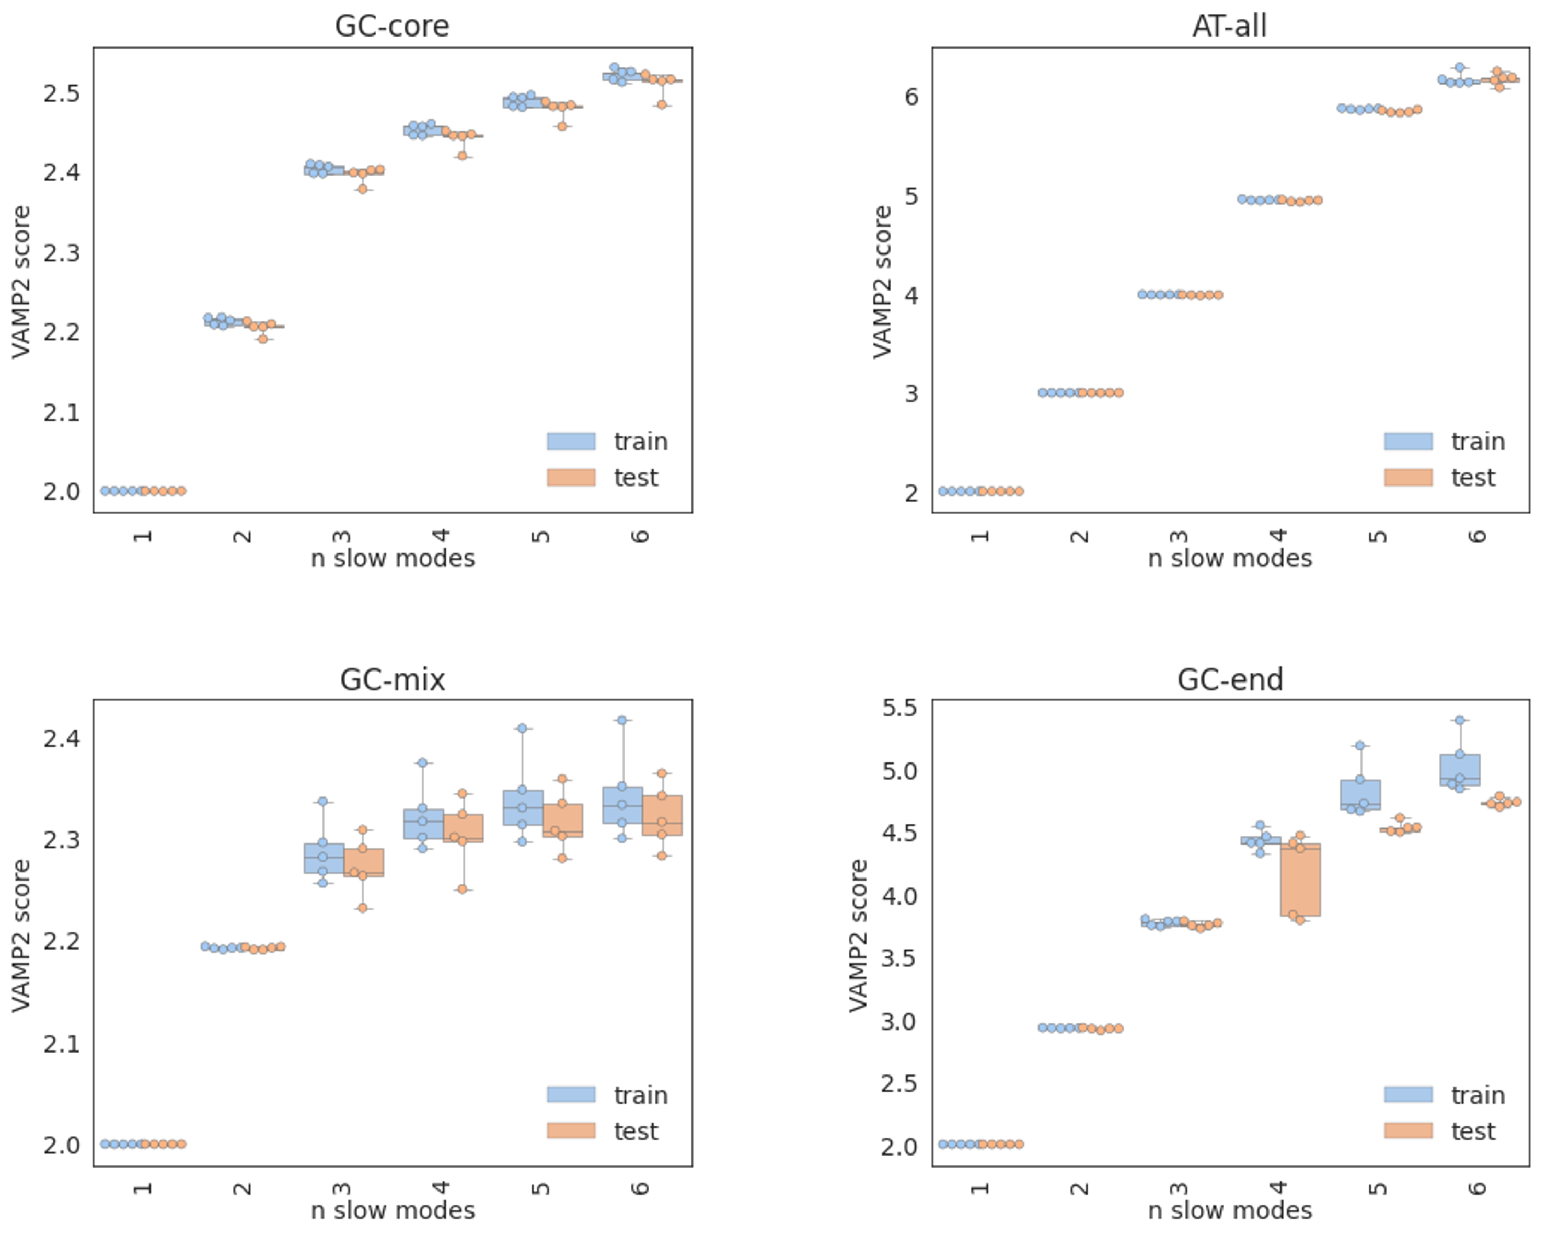
\includegraphics[width=1.0\textwidth]{FigS1.pdf}
        \caption{Five-fold cross-validation of the SRV VAMP-2 scores to select the optimal number of SRV coordinates for each sequence. A knee in the VAMP-2 plot was identified at the fifth, fourth, third, and second slow modes for AT-all, GC-end, GC-core, and GC-mix, respectively. An embedding of corresponding dimensionality was then used to cluster frames into discrete states. The absence of any significant separation in the training and testing VAMP-2 scores demonstrates that model is not overfitted.}
        \label{fig:SIFig1}
	\end{center}
\end{figure}

\clearpage
\newpage

% Fig. S2
\begin{figure}[ht!]
	\centering
    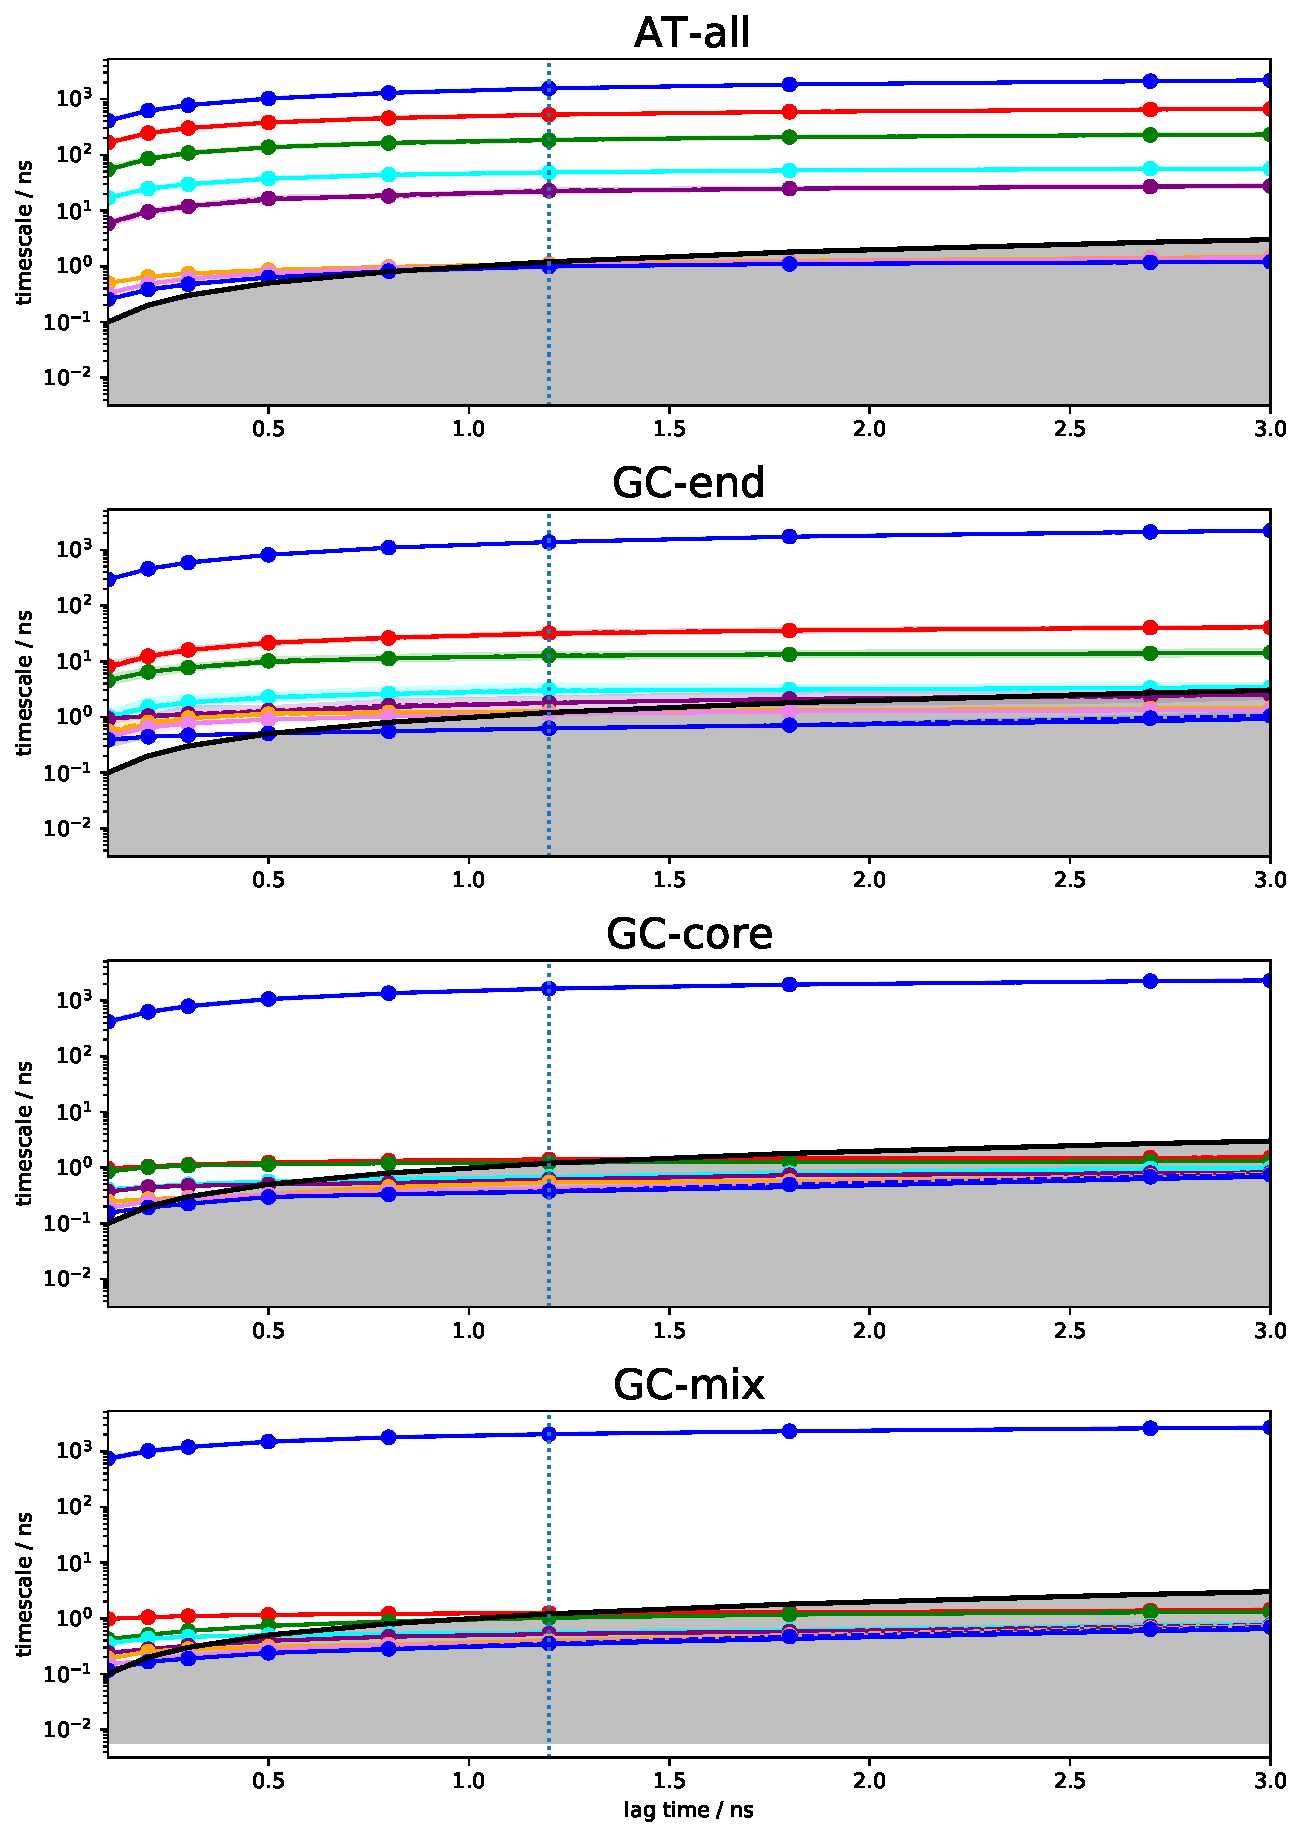
\includegraphics[width=0.75\textwidth]{FigS2.pdf}
    \caption{Convergence of the MSM implied time scales $t_i$ as a function of lag time $\tau$. Solid lines indicate maximum likelihood result while dashed lines show the Bayesian ensemble means superposed on shaded areas representing 95\% confidence intervals. The high simulation data volume used in our MSM construction means that the maximum likelihood and Bayesian ensemble means are in good agreement and confidence intervals are narrow. The implied time scales for all sequences converge at a lag time of $\tau$ = 1.2 ns (vertical line). The black solid curve marks equality of the implied time scale and lag time and delimits the shaded region wherein the implied time scales are shorter than the lag time and cannot be resolved.}
    \label{fig:SIFig2}
\end{figure}

\clearpage
\newpage

% Fig. S3
\begin{figure}[ht!]
	\begin{center}
        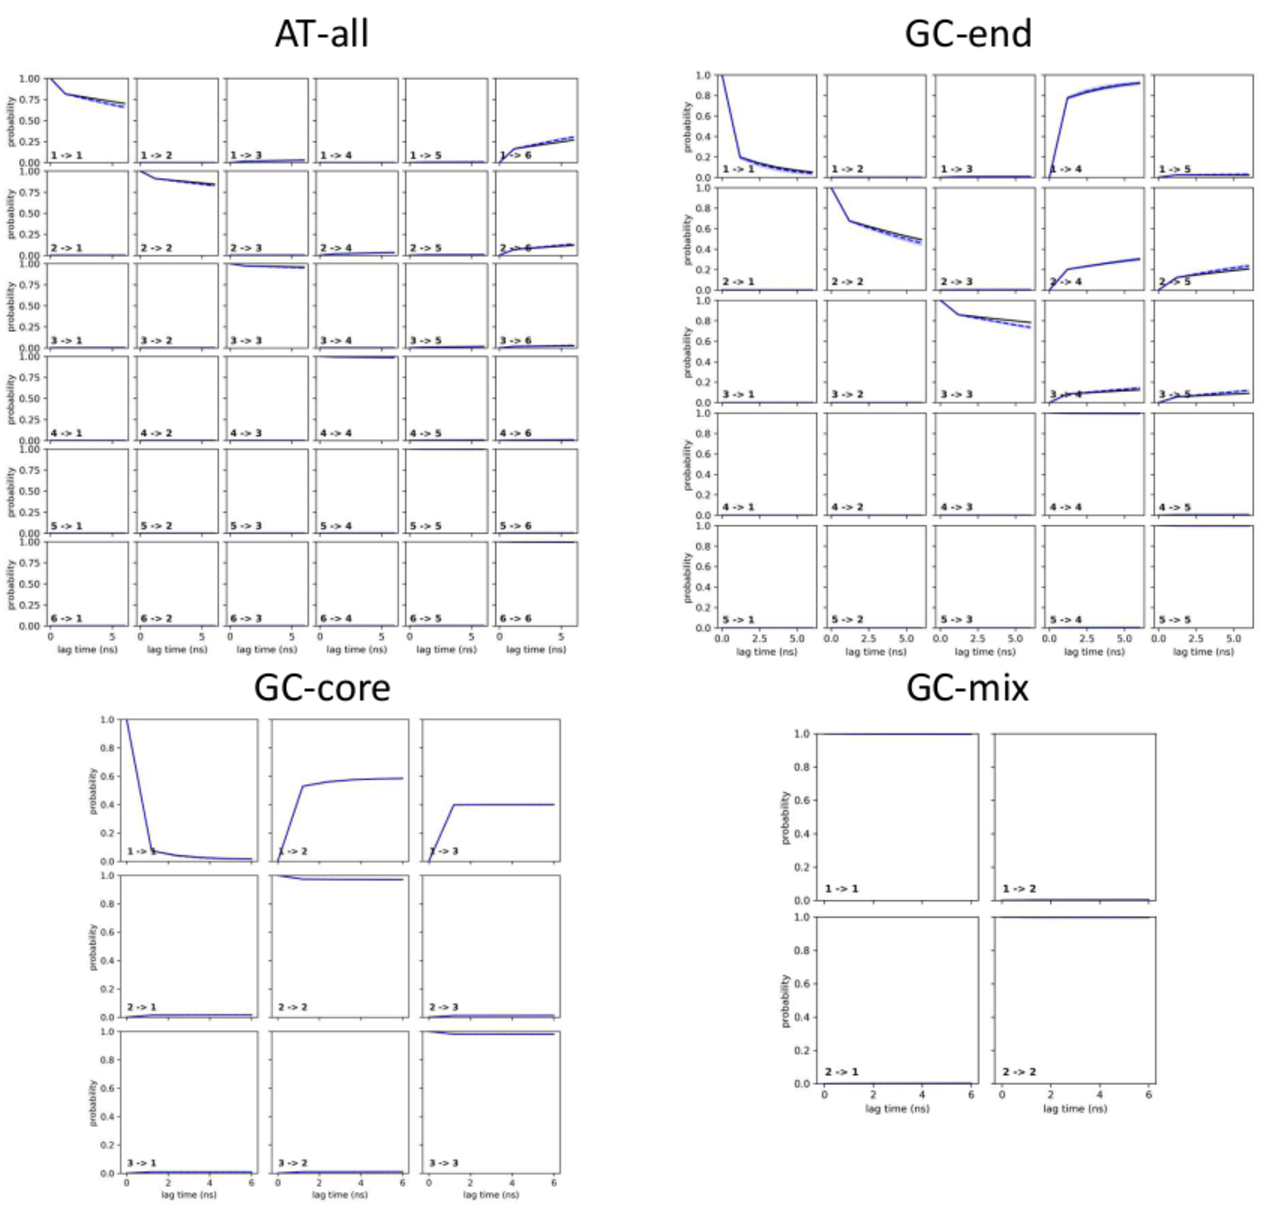
\includegraphics[width=1.0\textwidth]{FigS3.pdf}
        \caption{Chapman-Kolmogorov (CK) tests comparing the probabilities of remaining within each macrostates for each sequence as a function of lag time predicted by $k$ applications of an MSM constructed at the $\tau$ = 1.2 ns lag time $\mathbf{P}^k(\tau)$ (dashed blue line) versus those computed from an MSM constructed at that particular lag time $\mathbf{P}(k \tau)$ (solid black line). The blue shaded area indicates the estimated standard deviation in $\mathbf{P}^k(\tau)$. The good agreement between these two results provides numerical validation of the Markovian nature of the $\tau$ = 1.2 ns lag time MSM.}
        \label{fig:SIFig3}
	\end{center}
\end{figure}

\clearpage
\newpage

% Fig. S4
\begin{figure}[ht!]
	\centering
    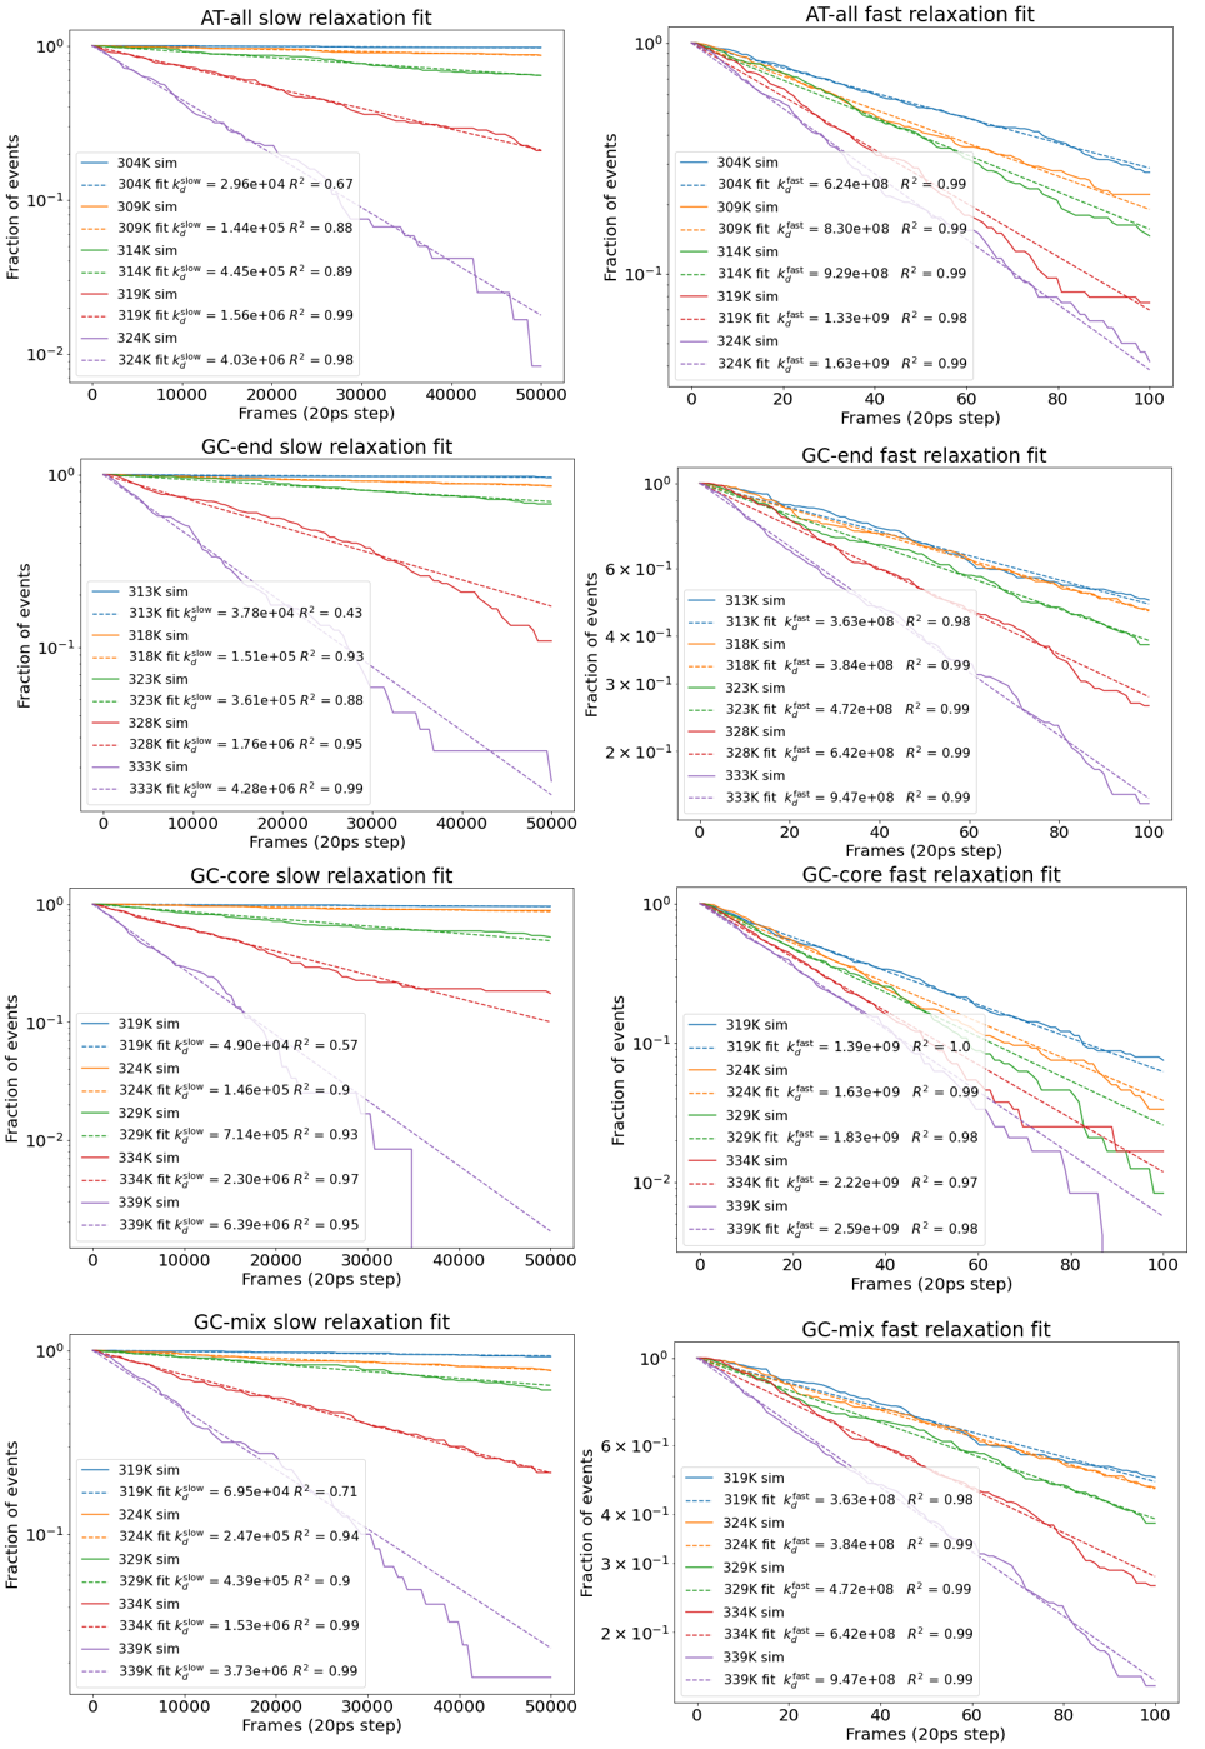
\includegraphics[width=.6\textwidth]{FigS4.pdf}
    \caption{Exponential fits for both slow (dissociation) and fast (fraying) response for all four sequences during ``computational T-jump'' experiments. From 120 independent 1 $\mu$s simulations, we compiled the slow response data by recording the fraction of sequences with both central Watson-Crick base pairs intact as a function of time, and the fast response data as the fraction of sequences with both terminal Watson-Crick base pairs intact as a function of time. We define a Watson-Crick base pair to be intact if the centers-of-mass of the two comlementary bases lie within a linear distance of 1.3 nm. We extracted our computational estimate of $k_d^\mathrm{fast}$ by fitting a decaying exponential to the fraction of bound A:T termini as a function of time $f_\mathrm{unfrayed}(t) = \exp(-k_d^\mathrm{fast}t)$. Similarly, we extracted our computational estimate of $k_d^\mathrm{slow}$ by fitting a decaying exponential to the fraction of hybridized sequences as a function of time $f_\mathrm{hybridized}(t) = \exp(-k_d^\mathrm{slow}t)$. \rood{We report within the figure legend to each panel the coefficient of determination $R^2$ for a least squares linear fit of the model to the data in log space (i.e., $\log \left( f \right) = -k_d t$) and data are plotted on log-linear axes to facilitate visual comparison of the fits. In all cases we observe excellent fits of the models to the data with all $R^2$ values equal to or better than 0.88 (except for the slow response at the the lowest temperature T$_m$-5K where dissociation events are sparse).}}
    \label{fig:SIFig4}
\end{figure}

\clearpage
\newpage

% Fig. S5
\begin{figure}[ht!]
	\centering
    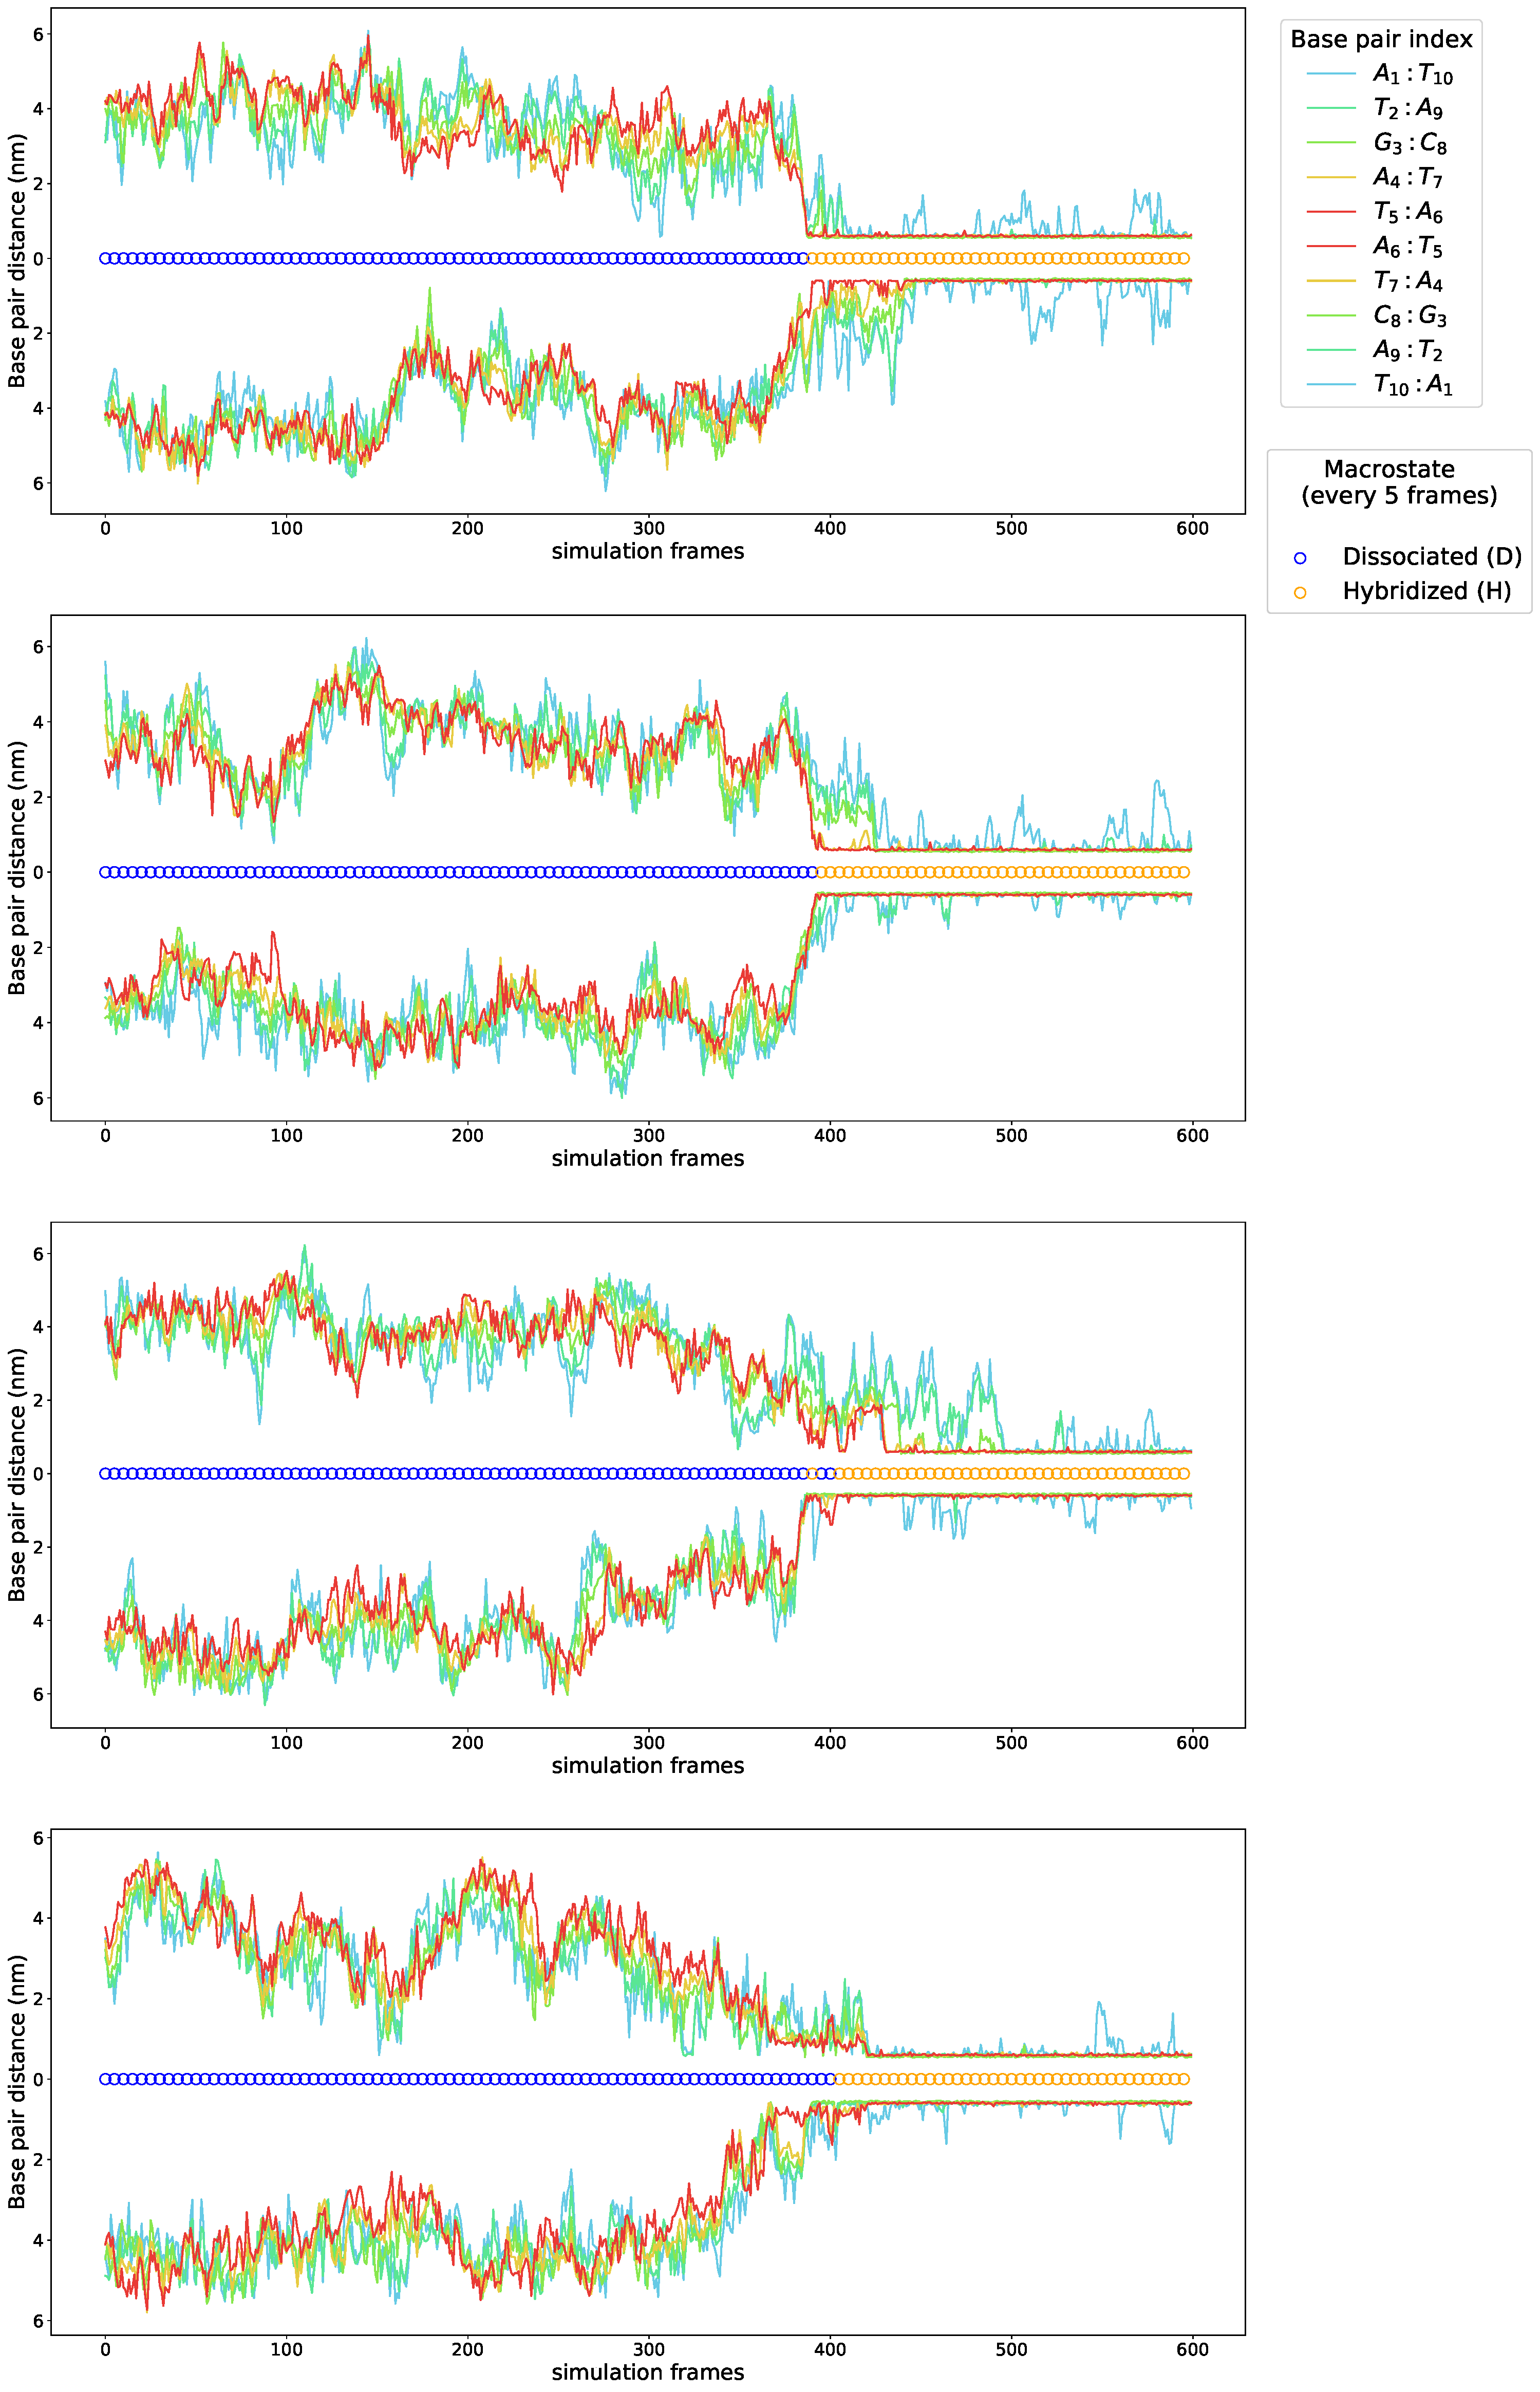
\includegraphics[width=0.8\textwidth]{FigS5a.pdf}
\end{figure}
\begin{figure}[ht!]
	\centering
    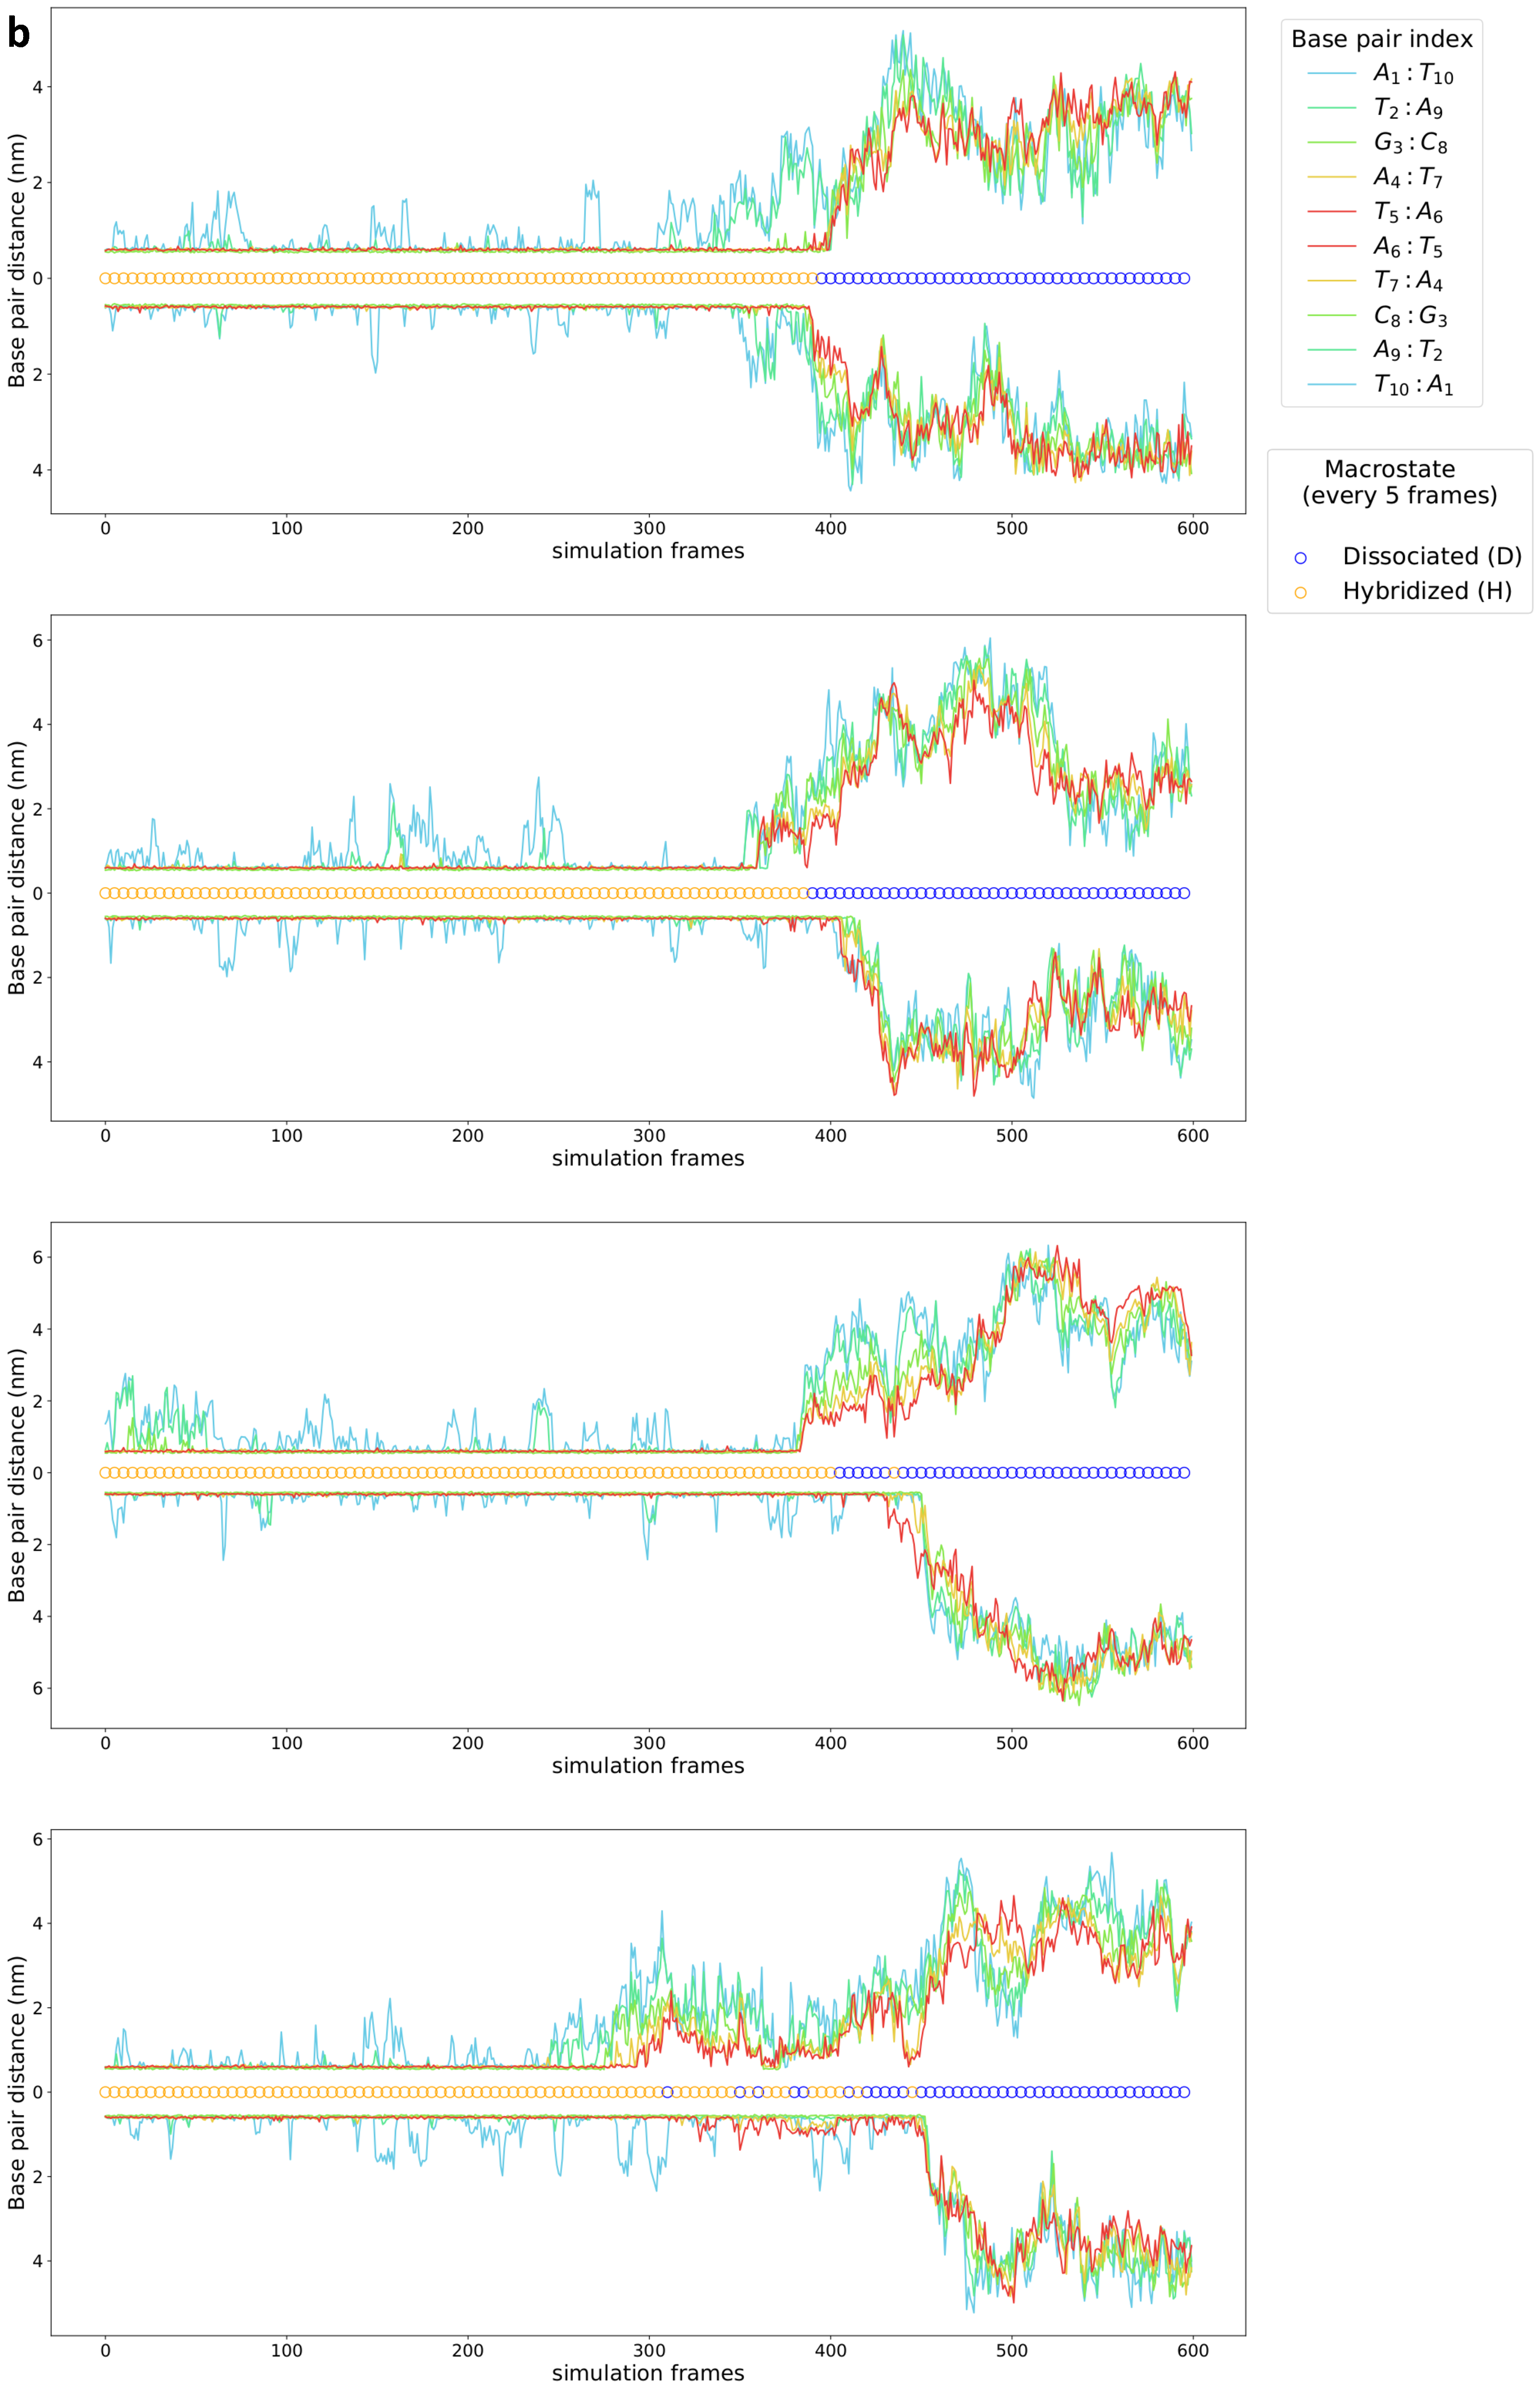
\includegraphics[width=0.8\textwidth]{FigS5b.pdf}
\end{figure}

\begin{figure}[ht!]
	\centering
    \caption{GC-mix hybridizes by nucleation-zippering and dehybridizes by fraying-peeling. Tracking of the 10 intermolecular distances between native WC base pairs over the course of four additional (a) hybridization and (b) dehybridization events. Symmetrically permutable distances (e.g., A$_1$:T$_{10}$ and T$_{10}$:A$_1$) are reflected across the x-axis to avoid congestion in the plot. Circles superposed on the x-axis indicate the instantaneous MSM state assignment as dissociated D (blue) or hybridized H (orange). Hybridization tends to occur by a nucleation-zippering mechanism, wherein a native G:C pair and adjacent A:T pair or 2-3 central A:T pairs first form prior to rapid formation of the duplex. Dehybridization tends to occur by a fraying-peeling mechanism wherein fraying of the two-base AT-tails on one or both sides of the duplex precedes dissociation of the central native base pairs and complete dissolution of the duplex.}
    \label{fig:SIFig5}
\end{figure}

\clearpage
\newpage

\subsection*{Nearest neighbor model of duplex thermodynamics}

DNA duplex hybridization thermodynamics are commonly predicted using nearest-neighbor (NN) models wherein the stability of a given base pair is assumed to solely depend on the identity and orientation of its adjacent base pairs. We apply the popular NN model reported by SantaLucia\citep{SantaLucia1998AThermodynamics} to estimate the stability of fully intact, shifted, and frayed duplex configurations observed in our MSMs. 

The NN model assumes hybridization proceeds in a two-state all-or-nothing manner. The Gibbs free energy difference between the hybridized and dissociated states can be determined from calculation of NN enthalpy and entropy contributions,
\begin{equation}\label{SIe1}
\Delta G_{NN}^{\circ}(T) = \Delta H_{NN}^{\circ} - T\Delta S_{NN}^{\circ}.
\end{equation}
$\Delta H_{NN}^{\circ}$ and $\Delta S_{NN}^{\circ}$ are assumed to be independent of temperature $T$, and are computed from the sum over all NN terms in a given configuration,
\begin{equation}\label{SIe2}
\Delta H_{NN}^{\circ} = \sum_{i}^{n_{NN}}\Delta H_{NN, i}^{\circ} + \sum_{j}^{n_{DE}}\Delta H_{DE, j}^{\circ} + \Delta H_{init}^{\circ},
\end{equation}
\begin{equation}\label{SIe3}
\Delta S_{NN}^{\circ} = \sum_{i}^{n_{NN}}\Delta S_{NN, i}^{\circ} + \sum_{j}^{n_{DE}}\Delta S_{DE, j}^{\circ} + \Delta S_{init}^{\circ} + \Delta S_{sym}^{\circ}.
\end{equation}                          
$\Delta H_{NN, i}^{\circ}$ is the NN enthalpy for a given dinucleotide step within duplex DNA, $\Delta H_{DE, j}^{\circ}$ corresponds to the enthalpic contribution from a given dangling end (DE) base next to the duplex\citep{Santalucia2004TheMotifs}, and $\Delta H_{init}^{\circ}$ is a duplex initiation term that accounts for terminal effects on duplex enthalpy. A schematic illustration of the NN and DE contributions for a fully hybridized duplex and an out-of-register shifted state is presented in Fig.~\ref{fig:SIFig6}. $\Delta S_{NN}^{\circ}$ is constructed in an analogous manner from NN, dangling end, and initiation terms, plus a symmetry term, $\Delta S_{sym}^{\circ}$, that applies an entropic penalty to self-complementary sequences for maintaining C2 symmetry. 

The SantaLucia NN parameters are defined for a solution condition at neutral pH with a sodium concentration of 1M. We use the empirical salt correction developed by Owczarzy\citep{Owczarzy2008PredictingCations} to determine the NN parameters at the sodium concentration used for simulations in this work. The Owczarzy model assumes the effect of counter-ions on DNA hybridization thermodynamics to be purely entropic,
\begin{equation}\label{SIe4}
\Delta S_{NN}^{\circ}(c_{Na^+}) = S_{NN}^{\circ}(1M) + \Delta H_{NN}^{\circ}[(4.29f_{GC}-3.95)\times 10^{-5} \ln{(c_{Na^+})}+ 9.4\times 10^{-6} (\ln{(c_{Na^+})})^2],
\end{equation} 
where $f_{GC}$ is the fractional G:C content of the duplex and $c_{Na^+}$ is the concentration of sodium counter-ions measured in M.  

\vspace{+0.5in}

\begin{figure}[ht!]
	\centering
    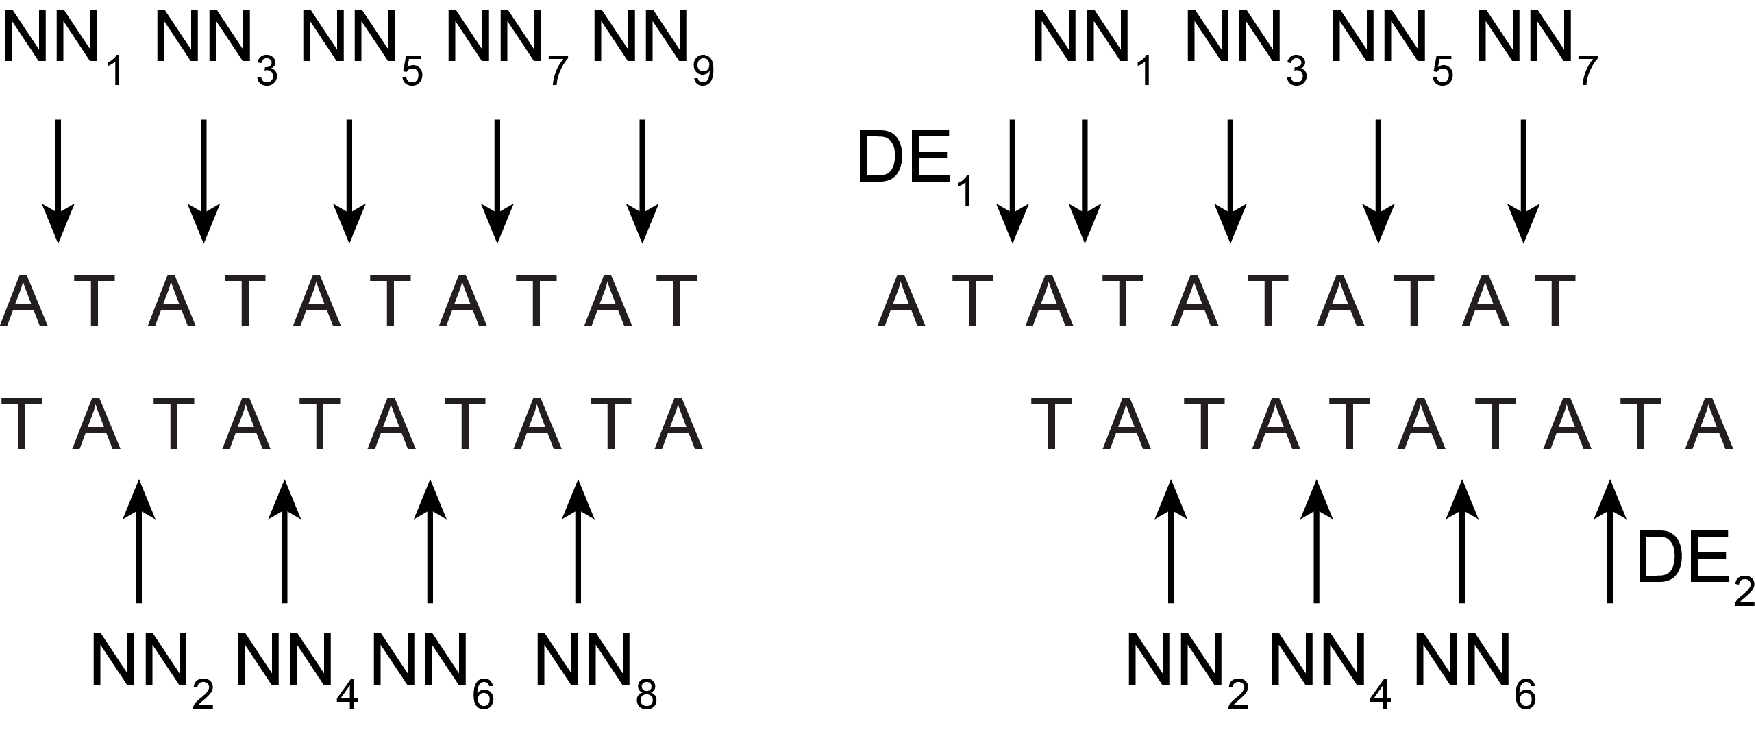
\includegraphics[width=.85\textwidth]{FigS6.pdf}
    \caption{Schematic of nearest neighbor (NN) contributions for a fully hybridized AT-all duplex and an out-of-register duplex with dangling ends (DE).}
    \label{fig:SIFig6}
\end{figure}

\clearpage
\newpage

\begin{figure}[ht!]
	\centering
    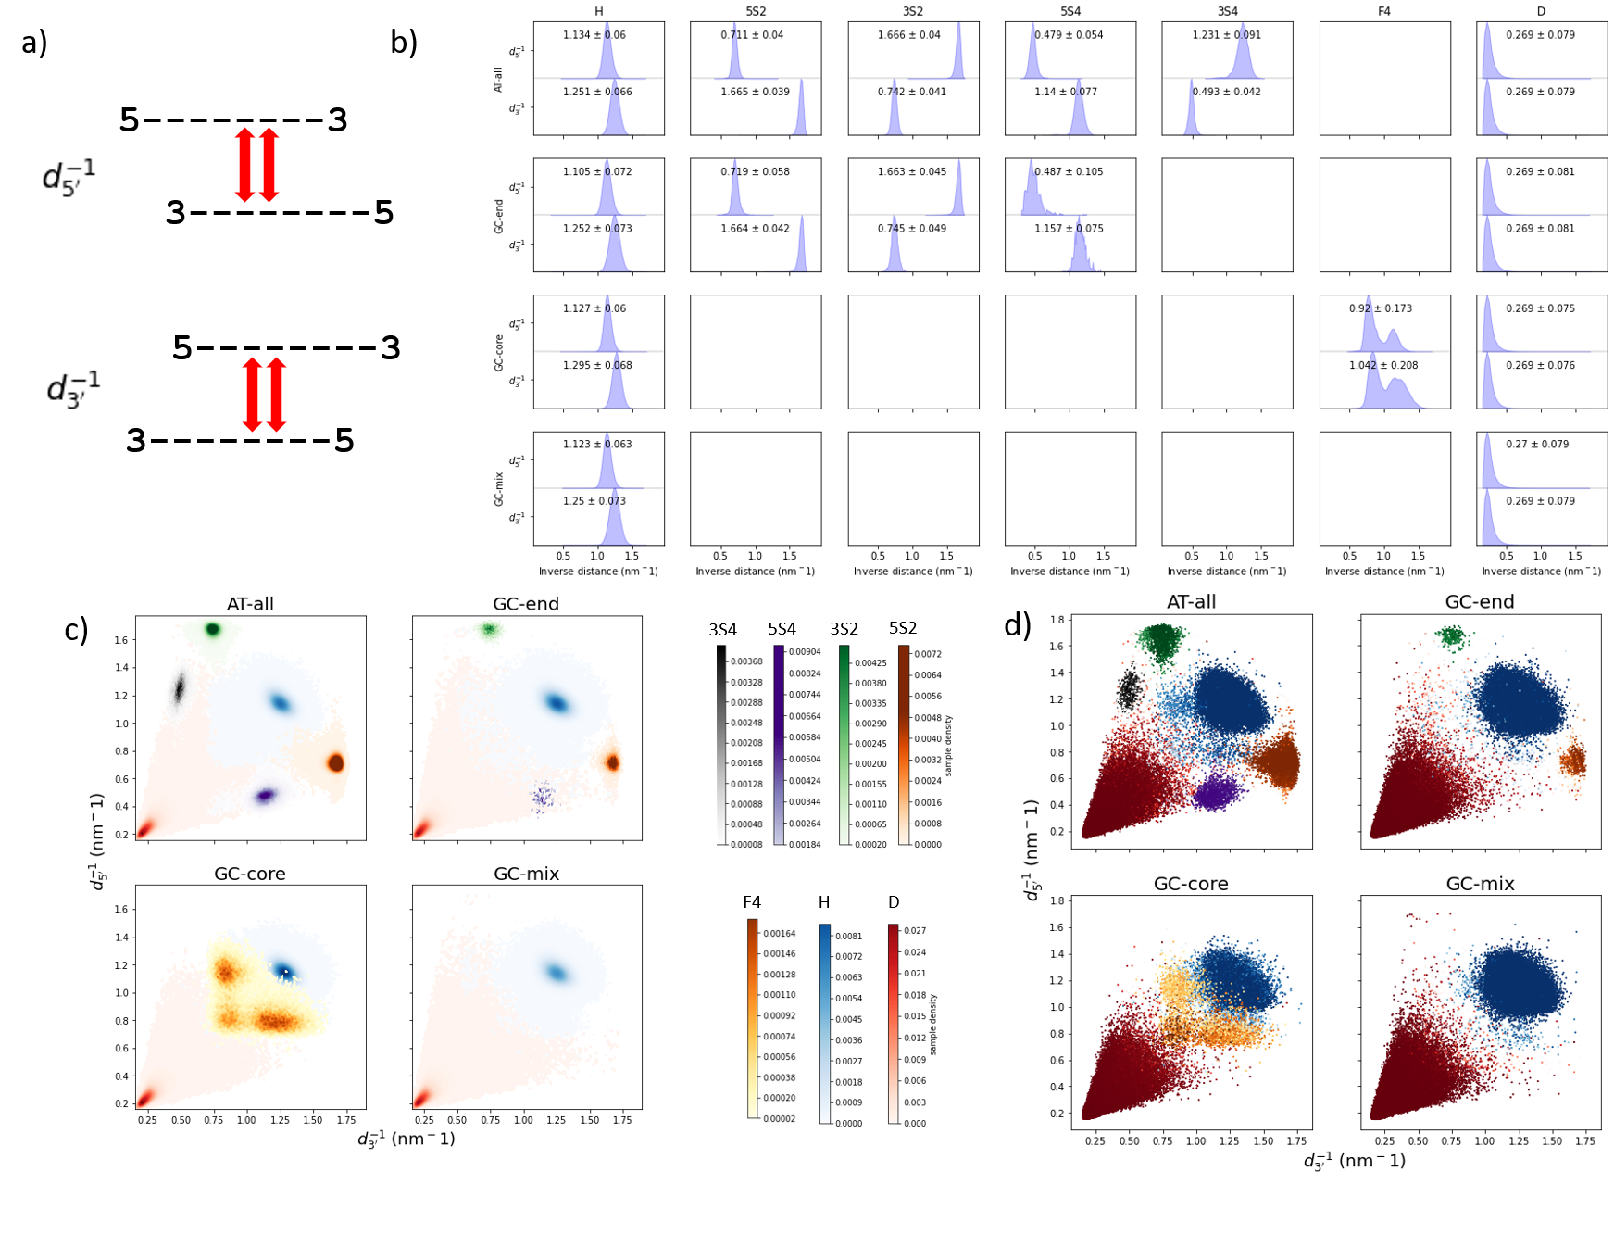
\includegraphics[angle=90,origin=c,width=1.0\textwidth]{FigS7.pdf}
\end{figure}

\begin{figure}[ht!]
	\begin{center}
        \caption*{\textbf{Figure S7.}\rood{Macrostate interpretation and structural analysis. The Markov state model macrostates are learned from the simulation trajectories using the featurization and deep learning procedure described in Section 2.1.2 of the main text, but it is informative to perform a \textit{post hoc} projection of the simulation data into a low-dimensional space spanned by physically interpretable order parameters in order to determine the structural characteristics of each macrostate and the structural heterogeneity of the microstate ensemble. (a) Definition of two physically-interpretable order parameters useful in characterizing the structure and base pairing of each microstate under both shifting and fraying. We define the $3^\prime$ shift for a particular base on a strand as the linear distance between that base and the base on the complementary strand offset by two base pairs in the $3^\prime$ direction. This distance reaches a minimum when the two strands are mutually shifted two base pairs in the $3^\prime$ direction. We define $d_{3^\prime}$ as the mean $3^\prime$ shift averaged over the two central bases, represented by red arrows, in the complementary strands. It is more convenient to work the reciprocal $d_{3^\prime}^{-1}$, since it has a finite range whereas $d_{3^\prime}$ diverges for dehybridized strands. We define $d_{5^\prime}^{-1}$ analogously as the reciprocal mean $5^\prime$ shift. We have found this pair of variables extremely informative in revealing the microstate and macrostate structure and base pairing patterns. (b) We report the mean and standard deviation of $d_{3^\prime}$ and $d_{5^\prime}$ taken over all microstates comprising each macrostate for each sequence. The small standard deviations that are consistent with a narrow distribution of the bulk of the microstates around the free energy minimum of each macrostate. (c) Superposition of sample density for each macrostate for each sequence AT-all, GC-end, GC-core, and GC-mix projected into $d_{3^\prime}^{-1}$-$d_{5^\prime}^{-1}$. This panel conveys two important pieces of information. First. each macrostate is anchored around a single free energy minimum containing the preponderance of the probability mass of the microstate ensemble. These projections indicate a relatively narrowly peaked distribution of microstates around the free energy minimum with a broad tail. Second, the location of each macrostate free energy minimum in the $d_{3^\prime}^{-1}$-$d_{5^\prime}^{-1}$ projection readily illuminates the base pair pattern within the duplex. Within the fully hybridized H state (blue) $d_{3^\prime}^{-1}$ $\approx$ $d_{5^\prime}^{-1}$ $\approx$ 1.2 nm$^{-1}$. A 2 b.p.\ shift to 3$^\prime$ is manifest in a decrease in $d_{3^\prime}^{-1}$ (increase in $d_{3^\prime}$) and a an increase in $d_{5^\prime}^{-1}$ (increase in $d_{5^\prime}$) producing the stable 3S2 state (green). A further 2 b.p.\ shift to 3$^\prime$ results in a further decrease in $d_{3^\prime}^{-1}$ and also a decrease in $d_{5^\prime}^{-1}$ (back down to the same value as in the H state) to produce the 3S4 state (black). Analogous arguments apply to the 2 b.p.\ 5$^\prime$ shifted state 5S2 (orange) and 4 b.p.\ 5$^\prime$ shifted state 5S4 (purple). The infinitely separated dehybridized state D exists at the origin, but limited by the finite box size corresponds to $d_{3^\prime}^{-1}$ $\approx$ $d_{5^\prime}^{-1}$ $\approx$ 0.2 nm$^{-1}$ (red). The GC-core frayed state F4 (orange) exists as a heart-shaped region between the H and D sates, with each symmetric lobe of the heart corresponding to fraying of one or other of the loose ends. (d) Coloring the microstates by their membership probabilities to their assigned macrostate under a fuzzy clustering procedure shows that microstates lying in the vicinity of the free energy minima have high probabilities whereas those at the macrostate cluster boundaries have less definitive assignments. The former comprise the preponderance of the microstate ensemble while the latter represent intermediate configurations that are transiently occupied as the system transitions from one macrostate to another.}}
        %\label{fig:macrostate_colors_FES}
	\end{center}
\end{figure}

\clearpage
\newpage




%\section{Supplemental Information}

% add secion on dmap and high temp methods?
%\subsection{Additional methods}

%\begin{figure}[ht!]
%	\begin{center}
%        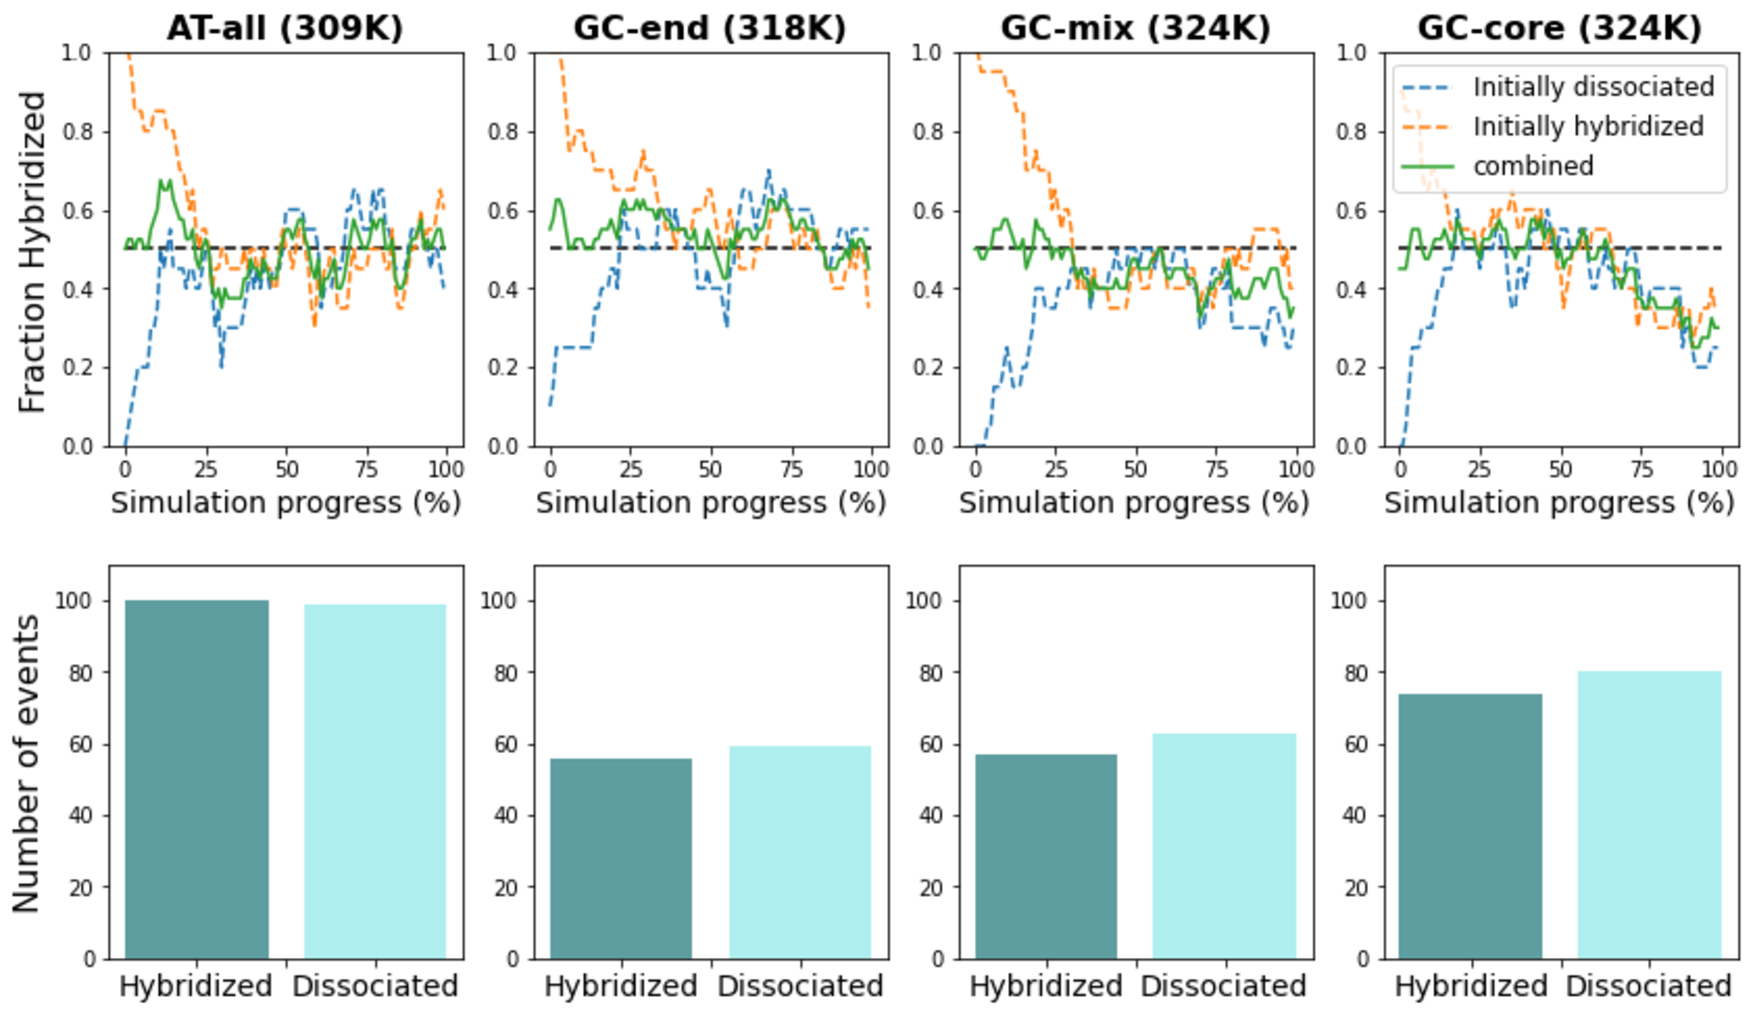
\includegraphics[width=0.9\textwidth, 
%        scale=0.5]{Figs/figs_imp/allseq_event_count.pdf}
%        \caption{All sequences consist of 20 trajectories initialized in the hybridized states and 20 in the dissociated state. Here we show fraction of hybridized duplexes averaged across these sets over time. For all sequences these curves converge near 0.5, but stochasticity of rare-event makes a definitive $T_m$ difficult to identify. The number of hybridization/dissocation combined across trajectories is shown. Not every trajectory contained a transition event, but on average more than one full event occurred (H$\rightarrow$D$\rightarrow$H) per trajectory, providing adequate sampling of dynamics. AT-all undergoes substantially more transition, but many of these do not reach a native (in-register) hybridized state. GC-core displays the most native hybridization events, perhaps due to stronger nucleation sites at the central G:C contact points.}
%        \label{fig:allseq_event_count}
%	\end{center}
%\end{figure}

% add figure for slow and fast response fitting (just GC-core)

%\subsection{VAMP-2 Scoring}
%The VAMP-2 score uses the covariances of a set of inputs to estimate the transfer operator of a dynamical system, providing a robust and object means to evaluate various parameters and models. Hyperparameters, including feature choice, number of microstates, and number of slow modes were evaluated and selection with via the VAMP-2 score. In the equations below, we show how covariances are obtained from some featurization $\chi$ of a time series $x_t$ and its time-lagged pairs $x_{t+\tau}$. The VAMP-2 score can then be found for $\chi$ by applying the VAMP principle with cross-validation.

%\begin{align*}
% 	\mathscr{C}_{00}=&\Expect{\chi(x_t)\chi(x_t)^\intercal}_t\\
% 	\mathscr{C}_{01}=&\Expect{\chi(x_t)\chi(x_{t+\tau})^\intercal}_t\\
% 	\mathscr{C}_{11}=&\Expect{\chi(x_{t+\tau})\chi(x_{t+\tau})^\intercal}_{t+\tau}\\
%	\\
% 	VAMP-2[\chi]=&\norm{\mathscr{C}_{00}^{-1/2}\mathscr{C}_{01}\mathscr{C}_{11}^{-1/2}}_F^2 +1
% 	%VAMP2^{val}[\chi]=&\norm{\mathscr{(C_{00}^{val})}^{-1/2}\mathscr{C}_{01}^{val}\mathscr({C}_{11}^{val})^{-1/2}}_F^2 + 1
%\end{align*}\label{CK1}

%\subsection{SRV hyperparameters}

%Using optimized hyperparameters and featurized trajectory data, we transformed 55 reciprocal pairwise distances into a low dimensional SRV basis set. In order to maintain consistency between sequences, we kept all SRV training hyperparameters the same with the exception of the number of outputed slow modes. We determined the number of slow modes via cross-validation on the VAMP-2 score to ensure that the coordinate did not over fit on statistical noise.\citep{McGibbon2015VariationalKinetics} In particular, we looked for convergence in the VAMP-2 score and inconsistency between cross validation scores -- suggesting that the model may be over-fitting on artifacts in the training data. We used a batch size of 50000 and ran each model for a total of 20 training epochs. We used two hidden layers and set the size of each layer to 100. For cross-validation and comparison between different hyper-parameters, we used a 80/20 validation split training. SRV training required about 22 GPU-minutes across 1 GPU and 10 CPUs. SRV training was implemented using Keras and Tensorflow.\citep{KerasGithub.Com, Abadi2016TensorFlow:Systems}

%\subsection{SRV-MSMs provide better resolution than tICA-MSMs} 

%\begin{figure}[ht!]
%	\begin{center}
%        \includegraphics[width=0.9\textwidth]{Figs/figs_imp/AT-all_implied_timescales.pdf}
%        \caption{SRV-MSM implied timescales converged faster than tICA-MSM implied across the five leading AT-all modes. Timescales are directly compared at the chose lag time of 1.2 ns}
%        \label{fig:AT-all_dynamic}
%	\end{center}
%\end{figure}

%\subsection{SRV-MSM walkthrough and analysis}

%In our analysis, we found that the AT-all sequence, given its repetitive structure and lack of GC-content, produced the most discernable spectral gap between modes. For this reason, we use this sequence a case study to work through our SRV-MSM pipeline step-by-step. Our first task was to identify the SRV lag time that was longer than the intrinsic Markov timescales of the system, yet short enough to resolve the dynamics of interest.\citep{Phys2018MarkovValidation} We found that an SRV lag time of 1.2 ns showed good convergence across the relevant timescales for all sequences. Next we selected an optimal number of SRV components to include in our analysis. After a certain point, higher order dynamical modes provide diminishing contributions the overall kinetic variance as measured by the Vamp-2 score, and the model can begin fitting on statistical noise in the trajectory data instead of the true dynamics.\citep{McGibbon2015VariationalKinetics} It is also more difficult to perform kmeans clustering on a high dimensional space, especially when those higher dimensions are less kinetically relevant.\citep{Pande2010EverythingAsk} For these reasons, the number of slow SRV components should be carefully selected based on the specific system of interest. As shown in figure \ref{fig:allseq_srv_crossval}), we see diminishing returns in the VAMP-2 score after five slow modes and select these modes as our optimized SRV basis.

%\subsubsection{SRV-MSM construction and optimization}
%Although SRV coordinates alone provide some information, we can access a more holistic picture of sequence kinetics and thermodynamics by using these SRV coordinates as a basis on which to construct an MSM. Because these coordinates are already capturing a majority of the system's kinetic variance, they serve as an ideal basis on which to group frames into microstates. We performed k-means clustering, and optimized the number of microstates at 200 by monitoring VAMP-2 score. Next, we selected an MSM lag time in a similar fashion to our SRV lag time selection process. This enables us to select a shorter lag time and build a higher resolution model than we could from an analogous tICA basis. Setting the MSM lag time to the same 1.2 ns we used for our SRVs, we built a Bayesian MSM to calculate transition probability matrix between each microstate. Finally, PCCA+ spectral clustering was implemented to group these microstates into macrostates that each represented a collection of metastable structures. Previous works have used a common set of microstates and/or performed manual clustering of microstates based on physical read outs from simulation data (stacking score, energies, etc).\citep{Pinamonti2017PredictingModels, PinamontiTheModels} Although these techniques are useful for performing comparisons between sequences, we saw better results when optimizing MSMs to capture the most detail of sequence individually and thus developed an independent set of microstates and macrostates for each sequence. 











%Next, we seek to interpret the physical relevance of these leading modes by plotting the Pearson correlation of each mode with the 100 intermolecular distances between strands. The quantitative meaning of these coordinates can be difficult to interpret given their nonlinear relationship to the SRV collective variables, but the relative different between these correlations shows which coordinates are most relevant to each process. For example, the first slow mode shows a positive correlation to each distance and the strongest correlation with native base pair distances (shown along the main diagonal). Given these correlations and the substantially longer timescale of this process, we can deduce that this leading mode corresponds to the overall hybridization and dissociation process. The next four SRV components all show a relatively high correlation along offset diagonals. These diagonals correspond to the intermolecular distances between complementary but out-of-register base pairs and point to the existence higher order ``shifting'' processes between sets of such base pairings. Previous ``inchworm'' and ``pseudoknot'' mechanisms have similarly been reported in simulation studies to correct base pair mismatches and occur on orders of magnitude longer timescales than underlying fast dynamics such as fraying.\citep{Romano2013DNADependence, Markegard2015, Maciejczyk2014DNAModel}

%We found GC-end had a similar implied timescales distribution to AT-all, with a distinct spectral gap after the fourth mode. For AT-all and GC-end, we kept to the convention of clustering into n+1 macrostates, where n is the number of slow components captured by the MSMs. For GC-core we built an SRV-MSM using these first three SRV modes as a basis and proceeded along the pipeline as described above. We found that four macrostate clustering was unstable -- likely because the third mode is mostly providing  information about dissociation dynamics -- so we performed PCCA+ clustering into three macrostates representing the hybridized (H), dissociated (D), and 4 4 base pair frayed (F4) states.  The GC-mix sequence showed a similar implied timescale distribution to GC-core, however we no longer saw a converged slow mode corresponding to multi-base fraying behavior. Instead, we observed two modes converge, corresponding to the association/dissociation dynamic and diffusive behavior while strands are dissociated. These correlate closely with the first and third GC-core SRV modes. Although we built our SRV-MSM using these two coordinates, we again were unable to form a stable third state along the second coordinate. As such, we designated this transitions as effectively two-state within the resolution of our model.

%For GC-core and GC-mix, we found this clustering convention to be unstable -- likely because the last converged mode was providing information about dissociation dynamics -- and performed PCCA+ with one less macrostate. 

%To visualize macrostates, we project the data into the two leading tICA coordinates. Although SRVs outperform these coordinates for the purpose of MSM construction, tICA coordinates represent good high variance collective variables on which to visualize free energies and state assignments.\citep{Sidky} Furthermore, we found that all macrostate were discernable on the first two tICA coordinates, whereas multiple SRV dimensions would be necessary to visualize states. After assigning these macrostates we calculated their stationary and transition probabilities averaged across 100 Gibbs sampled MSM and PCCA+ assignment. Means and standard deviations were calculated from this ensemble.

%As a preliminary check on SRV-MSM performance, we compared implied timescales with a more conventional tICA-MSM approach. Previous work showed that SRV-MSM implied timescales converged faster than tICA-MSM timescales, enabling a shorter lag time and therefore a higher resolution model.\citep{Sidky} Here we observed the same trend across all sequences, and we highlight these results for AT-all in figure \ref{fig:AT-all_dynamic}, emphasizing that faster convergence was observed across all leading timescales. Similar plots for the other sequences are included in the SI. We also note that the infrequency of transitions relative to the individual trajectory length leads to slower convergence of the leading mode. Because this mode corresponds the overall hybridization and dissociation process, we found that it displayed similar behavior across all sequences and that higher order modes were more informative for lag time selection.

%\subsection{SRV modes reveal hierarchical clustering structure}  % shift to include this in

%\begin{figure} %[ht!]
%	\begin{center}
%        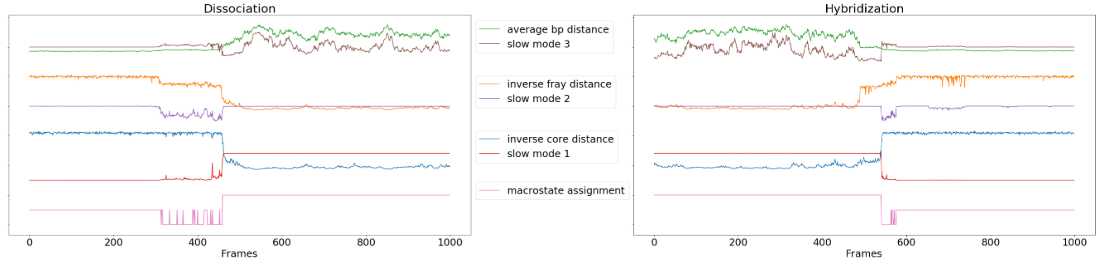
\includegraphics[width=0.8\textwidth]{Figs/figs_imp/GC-core_tracking_modes.pdf}
%        \caption{Leading GC-core SRV coordinates correlated with identifiable physical coordinates during sample hybridization (a) and dissociation (b) events. (c) Pearson correlations between all 100 intermolecular base pair distances and each the three leading slow modes. SRV2 correlations were calculated in the H and F4 states; SRV correlations were calculated in the D state.}
%        \label{fig:GC-core_tracking_modes}
%	\end{center}
%\end{figure}    

% not sure if this should directly follow the SRV-MSM GC-core description or directly follow the GC-core dmaps?
% try cutting this out entirely ?
%\subsection{SRV correlations to physical coordinates}

%Having constructed and interpreted SRV-MSMs, we revisited our original SRV basis to investigate how slow modes are constructed from input features. We found these GC-core modes to be of particular interest as they reveal the hierarchical and nonlinear nature of the dynamical encoding. We examined a collection of ``trimmed'' trajectories centered on both hybridization or dissociation events. For each trajectory, we compared the first three SRV coordinates with a corresponding collective variables with which they shared behavior. Two representative trajectories are shown in figure (\ref{fig:GC-core_tracking_modes}). Complementary G:C pairs are the best indicators for a hybridization/dissociation event, and we see a sharp change in the first SRV mode (SRV1) as these bonds form or break. The second slow mode (SRV2) is most active when G:C pairs are bound but the adjacent AT pairs are not. There is a small signal for fraying at the outer base pairs, but the mode overwhelmingly learns about these neighboring A:T/G:C bonds. Moreover, this behavior reflects movement in and out of the F4 state in the corresponding SRV-MSM discussed above. SRV3 is most active during dissociation, and seems to track closely with the average distance between all complementary base pairs. We attribute this to the SRV learning about the diffusive motions of the two body system and evaluating the likelihood of an imminent hybridization event. The third mode also peaks when the oligos are close together but configured in such a way that is not amenable hybridization. These misaligned conformations include inverse contacts where 5$^\prime$/5$^\prime$ and 3$^\prime$/3$^\prime$ ends meet and looped conformations where one strand is folded in on itself and preventing satisfactory WC contacts. 

%Despite the qualitative trends we observe between physical coordinates and leading SRV modes, we found it difficult to find correlations across full trajectories. With the exception of SRV1, Pearson correlations between physical coordinates and SRV modes were near zero and showed erroneous trends. However, when we performed this analysis along smaller sections of trajectories we noticed that the sign of SRV2 and SRV3 correlations switched depending on whether the oligos were in the hybridized or dissociated state. This shows that these modes are inherently nonlinear and provide support on top of the first mode -- which serves as an indicator function for hybridized vs. dissociated state. With respect to our SRV-MSM macroscates, we found that SRV2 was ``turned on'' in the H and F4 states -- corresponding to the intact helix and frayed state, respectively -- and SRV3 was turned on in the dissociated state. Accordingly, we calculated Pearson correlations between each SRV mode and all distances in states where the modes are active. Figure \label{fig:GC-core_tracking_modes} shows the highest correlation between SRV2 and inner A:T pairs, weak correlation with outer A:T pairs, and an inverse correlation with 5$^\prime$/5$^\prime$ and 3$^\prime$/3$^\prime$ pairs which tend to approach each when the duplex is in the F4 state. We also observed a highly symmetric correlation between SRV3 and central base pairs distances, which indicative of overall diffusive behavior. Taken together, these analyses reveal how the SRV learns and represents the dynamical space in an hierarchical manner, providing enhanced resolution to a linear method like tICA and producing the MSM results we observe above.

%\subsection{Structural diversity in the F4 state informs fraying dynamics} 



\clearpage
\newpage

\bibliography{references_210514_abv}

%%%%%%%%%%%%%%%%%%%%%%%%%%%%%%%%%%%%%%%%%%%%%%%%%%%%%%%%%%%%%%%%%%%%%
%% The "tocentry" environment can be used to create an entry for the
%% graphical table of contents.
%%%%%%%%%%%%%%%%%%%%%%%%%%%%%%%%%%%%%%%%%%%%%%%%%%%%%%%%%%%%%%%%%%%%%

%\clearpage


\end{document}
